\appendice
\chapter{Type-safe differentiable programming}

\section{Grammaire}\label{sec:kg_grammar}

Vous trouverez ci-dessous une grammaire BNF à peu près complète pour Kotlin$\nabla$ :

\newcommand{\mor}{\ensuremath{\;\mid\;}}
\newcommand{\code}[1]{\ensuremath{\text{\inline{#1}}}}
\newcommand{\bnfrl}[1]{\ensuremath{\langle#1\rangle}}
\allowdisplaybreaks
\begin{eqnarray*}
    \bnfrl{type} & ::= & \code{Double} \mor \code{Float} \mor \code{Int} \mor \code{BigInteger} \mor \code{BigDouble} \\
    \bnfrl{nat} & ::= & \code{1} \mor \ldots \mor \code{99} \\
    \bnfrl{output} & ::= & \code{Fun<}\bnfrl{type}\code{Real>} \mor \code{VFun<}\bnfrl{type}\code{Real,}\bnfrl{nat}\code{>} \mor \code{MFun<}\bnfrl{type}\code{Real,}\bnfrl{nat}\code{,}\bnfrl{nat}\code{>} \\
    \bnfrl{int} & ::= & \code{0} \mor \bnfrl{nat}\bnfrl{int} \\
    \bnfrl{float} & ::= & \bnfrl{int}\code{.}\bnfrl{int} \\
    \bnfrl{num} & ::= & \bnfrl{type}\code{(}\bnfrl{int}\code{)} \mor \bnfrl{type}\code{(}\bnfrl{float}\code{)} \\
    \bnfrl{var} & ::= & \code{x} \mor \code{y} \mor \code{z} \mor \code{ONE} \mor \code{ZERO} \mor \code{E} \mor \code{Var()} \\
\bnfrl{signOp} & ::= & \code{+} \mor \code{-} \\
\bnfrl{binOp} & ::= & \bnfrl{signOp} \mor \code{*} \mor \code{/} \mor \code{pow} \\
\bnfrl{trigOp} & ::= & \code{sin} \mor \code{cos} \mor \code{tan} \mor \code{asin} \mor \code{acos} \mor \code{atan} \mor \code{asinh} \mor \code{acosh} \mor \code{atanh} \\
\bnfrl{unaryOp} & ::= & \bnfrl{signOp} \mor \bnfrl{trigOp} \mor \code{sqrt} \mor \code{log} \mor \code{ln} \mor \code{exp} \\
\bnfrl{exp} & ::= & \bnfrl{var} \mor \bnfrl{num} \mor \bnfrl{unaryOp}\bnfrl{exp} \mor \bnfrl{var}\bnfrl{binOp}\bnfrl{exp} \mor \code{(} \bnfrl{exp} \code{)} \\
\bnfrl{expList} & ::= & \bnfrl{exp} \mor \bnfrl{exp} \code{,} \bnfrl{expList} \\
\bnfrl{linOp} & ::= & \bnfrl{signOp} \mor \code{*} \mor \code{ dot } \\
\bnfrl{vec} & ::= & \code{Vec(} \bnfrl{expList} \code{)} \mor \code{Vec} \bnfrl{nat} \code{(} \bnfrl{expList} \code{)} \\
\bnfrl{vecExp} & ::= & \bnfrl{vec} \mor \bnfrl{signOp}\bnfrl{vecExp} \mor \bnfrl{exp} \code{*} \bnfrl{vecExp} \mor \bnfrl{vec} \bnfrl{linOp} \bnfrl{vecExp} \mor \\
&&\bnfrl{vecExp}\code{.norm(}\bnfrl{int}\code{)} \\
\bnfrl{mat} & ::= & \code{Mat} \bnfrl{nat} \code{x} \bnfrl{nat} \code{(} \bnfrl{expList} \code{)} \\
\bnfrl{matExp} & ::= & \bnfrl{mat} \mor \bnfrl{signOp}\bnfrl{matExp} \mor \bnfrl{exp}\bnfrl{linOp}\bnfrl{matExp} \mor \\
&&\bnfrl{vecExp}\bnfrl{linOp}\bnfrl{matExp} \mor \bnfrl{mat} \bnfrl{linOp} \bnfrl{matExp} \\
\bnfrl{anyExp} & ::= & \bnfrl{exp} \mor \bnfrl{vecExp} \mor \bnfrl{matExp} \mor \bnfrl{derivative} \mor \bnfrl{invocation} \\
\bnfrl{bindings} & ::= & \bnfrl{exp} \code{ to } \bnfrl{exp} \mor \bnfrl{exp} \code{ to } \bnfrl{exp} \code{,} \bnfrl{bindings} \\
\bnfrl{invocation} & ::= & \bnfrl{anyExp} \code{(} \bnfrl{bindings} \code{)} \\
\bnfrl{derivative} & ::= & \code{d(} \bnfrl{anyExp} \code{) / d(} \bnfrl{exp} \code{)} \mor \bnfrl{anyExp} \code{.d(} \bnfrl{exp} \code{)} \mor \bnfrl{anyExp} \code{.d(} \bnfrl{expList} \code{)} \\
\bnfrl{gradient} & ::= & \bnfrl{exp} \code{.grad()}
\end{eqnarray*}

\chapter{Testing intelligent systems}

\section{Linear regression}\label{sec:lin_reg}

\noindent Rappeler l'équation matricielle de la régression linéaire (LR), où $\mathbf{X} : \mathbb{R}^{m \times n}$ et $\bm\Theta : \mathbb{R}^{n \times 1}$ :
%
\begin{equation}\label{eq:lin_reg}
\mathbf{\hat f}(\mathbf{X}; \bm\Theta) = \mathbf{X}\bm\Theta
\end{equation}
%
Imaginez que l'on nous donne l'ensemble de données suivant :
%
\begin{equation}
\mathbf{X} =
\begin{bmatrix}
\mathbf{x}_1 \\
\vdots \\
\mathbf{x}_m
\end{bmatrix} =
\begin{pmatrix}
1 & \ldots & x_{1n} \\
\vdots & \ddots & \vdots \\
1 & \ldots & x_{mn}
\end{pmatrix},
\mathbf{Y} =
\begin{bmatrix}
y_2 \\
\vdots \\
y_m
\end{bmatrix}
\end{equation}
%
Notre objectif en matière de moindres carrés ordinaires (OLS) LR est de minimiser la perte, ou l'erreur entre les données et la prédiction du modèle :
%
\begin{equation}
\mathcal{L}(\mathbf{X}, \mathbf{Y}; \bm\Theta) = ||\mathbf{Y} - \mathbf{\hat f}(\mathbf{X}; \bm\Theta)||^2
\end{equation}
%
\begin{equation}
\bm\Theta^* = \underset{\bm\Theta}{\operatorname{argmin}}\mathcal{L}(\mathbf{X}, \mathbf{Y}; \bm\Theta)
\end{equation}

\subsection{Méthode des différences finies}\label{sec:fdm}

Tout d'abord, nous considérons le cas scalaire, où $\mathbf{\hat f}(\mathbf{X} ; \bm\Theta) = \hat f(x ; \theta_2, \theta_1) = \theta_2 x + \theta_1$. Puisque $\mathbf{X}, \mathbf{Y}$ sont considérés comme fixes, nous pouvons réécrire $\mathcal{L}(\mathbf{X}, \mathbf{Y} ; \bm\Theta)$ aussi simplement :
%
\begin{equation}
\mathcal{L}(\bm\Theta) = \mathcal{L}(\theta_2, \theta_1) = \frac{1}{m}\sum_{i=1}^m(y_i - (\theta_2 x_i + \theta_1))^2
\end{equation}
%
Pour trouver le minimiseur de $\mathcal{L}(\bm\Theta)$, nous avons besoin de $\nabla_{\bm\Theta}\mathcal{L} = \lbrack \frac{\partial\mathcal{L}}{\partial \theta_2}, \frac{\partial\mathcal{L}{\partial \theta_1}\rbrack$. Il y a plusieurs façons de calculer cela. Tout d'abord, voyons les FDM avec des différences centrées :
%
\begin{align}
\frac{\partial\mathcal{L}}{\partial \theta_1} & = \underset{h \rightarrow 0}{\operatorname{lim}} \frac{\sum_{i=1}^m\left(y_i - \left(\theta_2 x_i + \theta_1 + h\right)\right)^2 - \sum_{i=1}^m\left(y_i - \left(\theta_2 x_i + \theta_1 - h\right)\right)^2}{2hm} \\ & = \underset{h \rightarrow 0}{\operatorname{lim}} \frac{1}{2hm}\sum_{i=1}^m\left(y_i - \left(\theta_2 x_i + \theta_1 + h\right)\right)^2 - \left(y_i - \left(\theta_2 x_i + \theta_1 - h\right)\right)^2 \label{eq:dL_dtheta0} \\
\frac{\partial\mathcal{L}}{\partial \theta_2} & = \underset{h \rightarrow 0}{\operatorname{lim}} \frac{\sum_{i=1}^m\left(y_i - \left((\theta_2 + h) x_i + \theta_1\right)\right)^2 - \sum_{i=1}^m\left(y_i - \left(\left(\theta_2 - h\right) x_i + \theta_1\right)\right)^2}{2hm} \\ & = \underset{h \rightarrow 0}{\operatorname{lim}} \frac{1}{2hm}\sum_{i=1}^m\left(y_i - \left(\left(\theta_2 + h\right) x_i + \theta_1\right)\right)^2 - \left(y_i - \left(\left(\theta_2 - h\right) x_i + \theta_1\right)\right)^2 \label{eq:dL_dtheta1}
\end{align}
%
En utilisant l'algèbre informatique, les équations ci-dessus peuvent être considérablement simplifiées :
%
\begin{align}
\frac{\partial\mathcal{L}}{\partial \theta_1} & = \underset{h \rightarrow 0}{\operatorname{lim}} \frac{1}{2hm}\sum_{i=1}^m\left(4h ( \theta_1 +  \theta_2 x_i - y_i)\right) \tag{\autoref{eq:dL_dtheta0} \href{https://www.wolframalpha.com/input/?i=(y_i-((\%CE\%B8_2\%2Bh)x_i\%2B\%CE\%B8_1))\%5E2-(y_i-((\%CE\%B8_2-h)x_i\%2B\%CE\%B8_1))\%5E2}{simplified}} \\
& = \boxed{\frac{2}{m}\sum_{i=1}^m\left(\theta_1 + \theta_2 x_i - y_i\right)} \\
\frac{\partial\mathcal{L}}{\partial \theta_2} & = \underset{h \rightarrow 0}{\operatorname{lim}} \frac{1}{2hm}\sum_{i=1}^m\left(4hx_i (\theta_2 x_i + \theta_1 - y_i)\right) \tag{\autoref{eq:dL_dtheta1} \href{https://www.wolframalpha.com/input/?i=(y_i-(\%CE\%B8_2*x_i\%2B\%CE\%B8_1\%2Bh))\%5E2\%E2\%88\%92(y_i-(\%CE\%B8_2*x_i\%2B\%CE\%B8_1-h))\%5E2}{simplified}} \\
& = \boxed{\frac{2}{m}\sum_{i=1}^m(x_i)(\theta_2 x_i + \theta_1 - y_i)}
\end{align}
%
%\begin{enumerate}
%\item[] \autoref{eq:dL_dtheta0}: \href{}
%\item[] \autoref{eq:dL_dtheta1}: \href{}
%\end{enumerate}

\subsection{Différenciation partielle}

\noindent Alternativement, nous pouvons calculer les partiels analytiquement, en appliquant la règle de la chaîne :
%
\begin{align}
\frac{\partial\mathcal{L}}{\partial \theta_1} & = \frac{\partial}{\partial \theta_1}\frac{1}{m}\sum_{i=1}^m(y_i - (\theta_2 x_i + \theta_1))^2 \\ & = \frac{1}{m}\sum_{i=1}^m 2 (y_i - (\theta_2 x_i + \theta_1))\frac{\partial}{\partial \theta_1}(y_i - (\theta_2 x_i + \theta_1)) \\ & = \frac{2}{m}\sum_{i=1}^m(y_i - (\theta_2 x_i + \theta_1))(-1) \\ & = \boxed{\frac{2}{m}\sum_{i=1}^m(\theta_2 x_i + \theta_1 - y_i)}
\end{align}
%
\begin{align}
\frac{\partial\mathcal{L}}{\partial \theta_2} & = \frac{\partial}{\partial \theta_2}\frac{1}{m}\sum_{i=1}^m(y_i - (\theta_2 x_i + \theta_1))^2 \\ & = \frac{1}{m}\sum_{i=1}^m 2(y_i - (\theta_2 x_i + \theta_1)) \frac{\partial}{\partial \theta_2}(y_i - (\theta_2 x_i + \theta_1)) \\ & = \frac{2}{m}\sum_{i=1}^m(y_i - (\theta_2 x_i + \theta_1))(-x_i) \\ & = \boxed{\frac{2}{m}\sum_{i=1}^m(x_i)(\theta_2 x_i + \theta_1 - y_i)}
\end{align}
%
Remarquez comment la différenciation analytique nous donne la même réponse que la \hyperref[sec:fdm]{méthode de la différence définie} (ce n'est pas un hasard), avec beaucoup moins d'algèbre. Nous pouvons réécrire ces deux solutions sous forme de gradient, c'est-à-dire comme un vecteur colonne de dérivées partielles :
%
\begin{equation}
\nabla_{\bm\Theta}\mathcal{L} =
\begin{bmatrix}
\frac{\partial\mathcal{L}}{\partial \theta_1} \\
\frac{\partial\mathcal{L}}{\partial \theta_2}
\end{bmatrix} = \frac{2}{m}
\begin{bmatrix}
\sum_{i=1}^m(\theta_2 x_i + \theta_1 - y_i) \\ \sum_{i=1}^m(x_i)(\theta_2 x_i + \theta_1 - y_i)
\end{bmatrix}
\end{equation}

\subsection{Matrix solution}\label{sec:linreg_matrix_sol}

Après avoir passé en revue la procédure scalaire pour LR, revenons maintenant à la forme générale de $\mathcal L(\bm\Theta)$. La notation matricielle nous permet de simplifier considérablement la perte :
%
\begin{align}
\mathcal L(\bm\Theta) & = \frac{1}{m} (\mathbf Y - \mathbf X \bm\Theta)^\intercal(\mathbf Y - \mathbf X \bm\Theta) \\ &= \frac{1}{m} (\mathbf Y^\intercal \mathbf Y - \mathbf Y^\intercal \mathbf X \bm\Theta - \bm\Theta^\intercal \mathbf X^\intercal \mathbf Y + \bm\Theta^\intercal \mathbf X^\intercal \mathbf X \bm\Theta) \\ &= \frac{1}{m} (\mathbf Y^\intercal \mathbf Y - 2 \bm\Theta^\intercal \mathbf X^\intercal \mathbf Y + \bm\Theta^\intercal \mathbf X^\intercal \mathbf X \bm\Theta)
\end{align}
%
La notation matricielle nous permet de dériver le gradient et nécessite beaucoup moins d'algèbre :
%
\begin{align}
\nabla_{\bm\Theta}\mathcal L(\bm\Theta) & = \frac{1}{m} (\nabla_{\bm\Theta}\mathbf Y^\intercal \mathbf Y - 2 \nabla_{\bm\Theta} \bm\Theta^\intercal \mathbf X^\intercal \mathbf Y + \nabla_{\bm\Theta}\bm\Theta^\intercal \mathbf X^\intercal \mathbf X \bm\Theta) \\ & = \frac{1}{m} ( 0 - 2\mathbf{X}^\intercal \mathbf Y + 2 \mathbf{X}^\intercal \mathbf X \bm\Theta ) \\ & = \boxed{\frac{2}{m} (\mathbf{X}^\intercal \mathbf X \bm\Theta - \mathbf{X}^\intercal \mathbf Y)}
\end{align}
%
Pour être complet, et pour nous en convaincre, la solution matricielle est en effet la même :
%
\begin{align}
& = \frac{2}{m}\left(
\underbrace{\begin{bmatrix}
1 & \ldots & 1 \\
x_1 & \ldots & x_m \\
\end{bmatrix}}_{\mathbf{X}^\intercal}
\underbrace{\begin{bmatrix}
1 & x_1 \\
\vdots & \vdots \\
1 & x_m
\end{bmatrix}}_{\mathbf{X}}
\underbrace{\begin{bmatrix}
\theta_1 \\
\theta_2
\end{bmatrix}}_{\bm\Theta} -
\underbrace{\begin{bmatrix}
1 & \ldots & 1 \\
x_1 & \ldots & x_m \\
\end{bmatrix}}_{\mathbf{X}^\intercal}
\underbrace{\begin{bmatrix}
y_1 \\
\vdots \\
y_m
\end{bmatrix}}_{\mathbf{Y}}\right) \\
& = \frac{2}{m}\left(
\underbrace{\begin{bmatrix}
m & \sum_{i=1}^{m}x_i \\
\sum_{i=1}^{m}x_i & \sum_{i=1}^{m}x_i^2 \\
\end{bmatrix}}_{\mathbf{X}^\intercal\mathbf{X}}
\underbrace{\begin{bmatrix}
\theta_1 \\
\theta_2
\end{bmatrix}}_{\bm\Theta} -
\underbrace{\begin{bmatrix}
\sum_{i=1}^{m}y_i \\
\sum_{i=1}^{m}x_iy_i
\end{bmatrix}}_{\mathbf{X}^\intercal\mathbf{Y}}\right) \\
& = \frac{2}{m}\left(
\underbrace{\begin{bmatrix}
m \theta_1 + \sum_{i=1}^{m}\theta_2x_i \\
\sum_{i=1}^{m}\theta_1x_i + \sum_{i=1}^{m}\theta_2x_i^2
\end{bmatrix}}_{\mathbf{X}^\intercal\mathbf{X}\bm\Theta} -
\underbrace{\begin{bmatrix}
\sum_{i=1}^{m}y_i \\
\sum_{i=1}^{m}x_iy_i
\end{bmatrix}}_{\mathbf{X}^\intercal\mathbf{Y}}\right) \\
& = \boxed{\frac{2}{m}
\underbrace{\begin{bmatrix}
\sum_{i=1}^{m}\theta_2x_i + \theta_1 - y_i \\
\sum_{i=1}^{m}(x_i)(\theta_2x_i + \theta_1 - y_i)
\end{bmatrix}}_{\mathbf{X}^\intercal\mathbf{X}\bm\Theta - \mathbf{X}^\intercal\mathbf{Y}} =
\begin{bmatrix}
\frac{\partial\mathcal{L}}{\partial \theta_1} \\
\frac{\partial\mathcal{L}}{\partial \theta_2}
\end{bmatrix} = \nabla_{\bm\Theta}\mathcal{L}(\bm\Theta)}
\end{align}
%
Remarquez comment nous récupérons la même solution obtenue par différenciation partielle et approximation par différence finie, bien que sous une forme plus compacte. Pour une bonne introduction au calcul matriciel, le manuel de \citet{magnus2019matrix} est un excellent guide, dont \citet{petersen2012matrix} offre une revue des identités importantes.

Les SLO LR sont un problème d'optimisation convexe. Si $\mathbf X^\intercal \mathbf X$ est inversible, c'est-à-dire de plein rang, cela implique une solution unique $\bm\Theta^*$, que nous pouvons résoudre directement en fixant $\nabla_{\bm\Theta}\mathcal{L} = \mathbf{0}$ :
%
\begin{align}\label{eq:norm_eq}
\mathbf{0} & = \mathbf X^\intercal \mathbf X \bm \Theta - \mathbf X ^ \intercal \mathbf Y \\ \bm\Theta &= (\mathbf X^\intercal \mathbf X)^{-1}\mathbf X^\intercal\mathbf Y
\end{align}
%
Pour résoudre ce problème, il faut calculer $(\mathbf{X}^\intercal\mathbf{X})^{-1}$, soit au moins $\mathcal{O}(n^{2.373})$\citep{williams2014multiplying}, c'est-à-dire quadratique par rapport au nombre de dimensions d'entrée. Une autre façon de trouver $\bm \Theta^*$ consiste à initialiser $\bm\Theta \leftarrow \mathbf{0}$ et à répéter la procédure suivante jusqu'à la convergence :
%
\begin{equation}
\bm\Theta' \leftarrow \bm\Theta - \alpha \nabla_{\bm\Theta}\mathcal L(\bm\Theta)
\end{equation}
%
Généralement, $\alpha \in [0.001, 0.1]$. Bien qu'un réglage des hyperparamètres soit nécessaire pour trouver un $\alpha$ approprié (diverses améliorations comme le moment de Nesterov~\citep{nesterov2013gradient} et les méthodes quasi-Newton contribuent également à accélérer la convergence), cette procédure est garantie d'être plus efficace sur le plan des calculs que l'inversion de la matrice pour des $m$ et $n$ suffisamment importants. En pratique, l'équation normale~\autoref{eq:norm_eq} est rarement utilisée, sauf si $m$ est très petit.

\section{Régression polynomiale}\label{sec:poly_reg}

\subsection{Univariate PR}

La régression polynomiale est une application simple de la LR, dans laquelle nous approximons les coefficients pour chaque terme dans un polynôme scalaire. Considérons le cas univarié :

\begin{equation}
y_i \,=\, \beta_0 + \beta_1 x_i + \beta_2 x_i^2 + \cdots + \beta_m x_i^m = \sum_{j=0}^{m} \beta_j x_i^{j}
\end{equation}
%
Nous pouvons réécrire cette fonction sous forme de matrice comme suit :
%
\begin{equation}
\begin{bmatrix} y_1\\ y_2\\ y_3 \\ \vdots \\ y_n \end{bmatrix}= \begin{bmatrix} 1 & x_1 & x_1^2 & \dots & x_1^m \\ 1 & x_2 & x_2^2 & \dots & x_2^m \\ 1 & x_3 & x_3^2 & \dots & x_3^m \\ \vdots & \vdots & \vdots & \ddots & \vdots \\ 1 & x_n & x_n^2 & \dots & x_n^m \end{bmatrix} \begin{bmatrix} \beta_0\\ \beta_1\\ \beta_2\\ \vdots \\ \beta_m \end{bmatrix}
\end{equation}
%
\begin{equation}
\mathbf{\hat f}(\mathbf{X}; \bm\beta) = \mathbf{X}\bm\beta
\end{equation}
%
La ressemblance avec \autoref{eq:lin_reg} devrait être claire. Pour trouver $\bm\beta$ en minimisant $\mathcal L(\mathbf{X}, \mathbf{Y};\bm\beta)$, nous pouvons utiliser la même méthode décrite dans \autoref{sec:linreg_matrix_sol}. Ici, $\mathbf x, \mathbf y \in \mathbb R^n$, où $(x_i, y_i)$ correspondent à des points scalaires dans notre ensemble de données de taille $n$. La matrice $\mathbf X \in \mathbb R^{n \times m}$ représente une \textit{fonction map}, $\varphi : \mathbb R \rightarrow \mathbb R^m$, appliquée par éléments à chaque valeur d'entrée $x_i$ dans notre ensemble de données, où $\varphi(x_i) = \left[1, x_i^2, \ldots, x_i^m\right]$.

\subsection{Multivariate PR}

Dans la RP multivariée, nous avons besoin de coefficients pour toutes les interactions par paires entre chaque variable et chaque autre à chaque degré du polynôme. Considérons le cas bivarié :
%
\begin{equation}
    y_i(\mathbf w, \mathbf x) = 1 + \beta_{\mathbf x} \mathbf x + \beta_{\mathbf w}\mathbf w + \beta_{\mathbf x\mathbf w} \mathbf x\mathbf w + \beta_{\mathbf x^2} \mathbf x^2 + \beta_{\mathbf w^2} \mathbf w^2 + \beta_{\mathbf x\mathbf w^2} \mathbf x\mathbf w^2 + \cdots + \beta_{\mathbf w^m\mathbf x^m} \mathbf w^m\mathbf x^m
\end{equation}
%
Cela nécessite au moins $(n \times m \times 2)$ termes. Minimiser $\bm\beta$ sur cette expression devient directement insoluble car le degré maximum $m$, la taille de l'ensemble de données $n$ et le nombre de variables augmentent.

\subsection{Kernel trick}

Au lieu de modéliser $\mathbf X$ explicitement, construisons une fonction spéciale $k : \langle\varphi(\mathbf x), \varphi(\mathbf w)\rangle \mapsto \mathbb R$, où $k(\mathbf w, \mathbf x) = (1 + \mathbf w^\intercal \mathbf x)^2$. Appelée \textit{noyau}, cette fonction fait partie d'une famille bien étudiée de \textit{fonctions-noyau}, $K : \Omega \times \Omega \rightarrow \mathbb R$ avec une structure supplémentaire. En écrémant les détails, un noyau valide préserve le produit intérieur dans notre espace de fonctionnalité. Pour plus de simplicité, laissez $\mathbf w, \mathbf x \in \mathbb R^2$. Supposons que nous ayons une carte des caractéristiques $\varphi(\mathbf v) = \left[1, v_1^2, v_2^2, \sqrt{2} v_1, \sqrt{2} v_2, \sqrt{2} v_1 v_2\right]$. Nous observons :

\begin{align}\label{eq:feature_map}
    k(\mathbf w, \mathbf x) &= \varphi(\mathbf w) \varphi(\mathbf x) \\
    &=[1, w_1^2, w_2^2, \sqrt{2} w_1, \sqrt{2} w_2, \sqrt{2} w_1 w_2]\begin{bmatrix}
                                                                                   1\\ x_1^2\\ x_2^2\\ \sqrt{2} x_1\\ \sqrt{2} x_2\\ \sqrt{2} x_1 x_2
    \end{bmatrix}\\
    & = \boxed{1 + w_1^2 x_1^2 + w_2^2 x_2^2 + 2 w_1 x_1 + 2 w_2 x_2 + 2 w_1 w_2 x_1 x_2}
\end{align}
%
En développant le noyau $k(\mathbf w, \mathbf x)$ comme suit :
%
\begin{align}
k(\mathbf w, \mathbf x) & = (1 + \mathbf w^\intercal \mathbf x)^2 = (1 + w_1 \, x_1 + w_2 \, x_2)^2 \\
& = \boxed{1 + w_1^2 x_1^2 + w_2^2 x_2^2 + 2 w_1 x_1 + 2 w_2 x_2 + 2 w_1 w_2 x_1 x_2}
\end{align}
%
Nous récupérons \autoref{eq:feature_map} sans utiliser directement $\varphi$. C'est ce qu'on appelle le \textit{kernel trick}, une technique largement utilisée dans de nombreux domaines de l'apprentissage machine.

\chapter{Tools for reproducible robotics}

\section{Useful Docker resources}

Les ressources suivantes se sont avérées particulièrement utiles lors du développement de l'infrastructure de conteneurs de Duckietown.

\subsection{\href{https://www.balena.io/}{Balena}}\label{subsec:balena}

Balena est une très bonne source d'images de base pour les appareils ARM. La meilleure utilisation des images Balena est qu'elles peuvent être reconstruites sur des appareils x86, tels qu'un ordinateur portable ou un serveur en nuage. Chaque image Balena contient une cale pour le shell qui permettra aux utilisateurs d'exécuter des binaires ARM sur x86 depuis l'intérieur d'un conteneur. Pour utiliser cette fonctionnalité, le modèle \inline{Dockerfile} suivant est fourni :
%
\begin{dockerlisting}
FROM balena/BASE_IMAGE # e.g. raspberrypi3-python
RUN [ "cross-build-start" ]
# ARM-specific code goes here...
RUN [ "cross-build-end" ]
CMD <DEFAULT_START_COMMAND>
\end{dockerlisting}
%
Balena utilise \href{https://www.qemu.org/}{QEMU}~\citep{bellard2005qemu} pour croiser les images.\hspace{-.08em}\footnote{\url{https://www.balena.io/blog/building-arm-containers-on-any-x86-machine-even-dockerhub/}} Lorsque vous exécutez une image ARM, utilisez simplement le binaire \inline{qemu-arm-static} comme point d'entrée personnalisé :
%
\begin{pclisting}
~$ docker run (*@\hl{--entrypoint=qemu-arm-static}@*) -it your/arm-image bash
\end{pclisting}

\subsection{\href{https://hub.docker.com/_/ros}{ROS Docker Images}}

ROS.org construit des images ARM et x86 nocturnes pour le développement de la robotique. Pour chaque distribution, il existe des paquets comme \inline{core}, \inline{base}, \inline{perception} (y compris \href{https://opencv.org/}{OpenCV}), \inline{robot} et autres.\vspace{10pt}
%
\begin{centering}
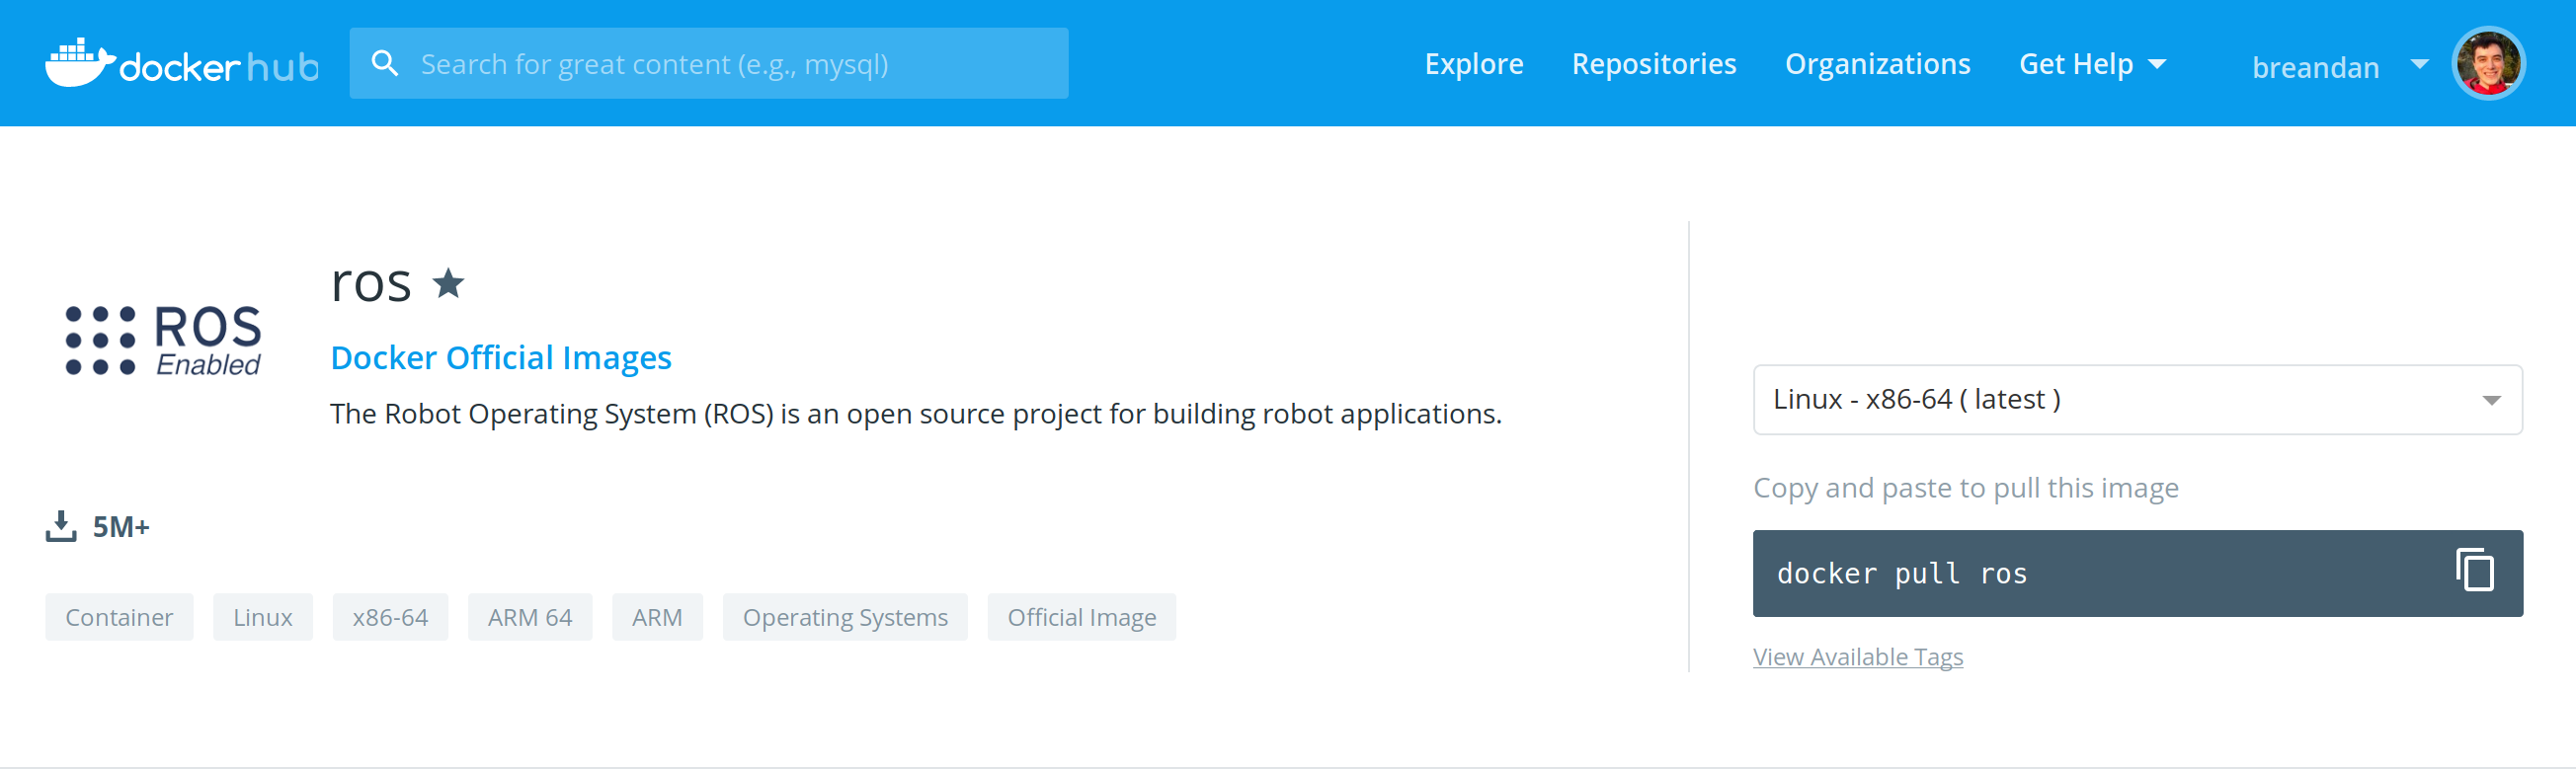
\includegraphics[width=\textwidth]{../figures/ros_docker_images.png}
\end{centering}

\subsection{\href{https://blog.hypriot.com/}{Hypriot}}\label{subsec:hypriot}

Hypriot, un OS de base pour RPi et autres dispositifs ARM, inclut le support de Docker dès sa sortie de la boîte. Hypriot est une distribution Linux légère basée sur Raspbian qui \href{https://github.com/hypriot/image-builder-rpi}{construit} à partir des derniers noyaux Pi de Raspberry et des dernières versions de Raspbian.

\subsection{\href{https://www.piwheels.org/}{PiWheels}}

Tous les paquets Python (surtout s'ils contiennent une bibliothèque native) ne peuvent pas être exécutés sur toutes les plates-formes. On pourrait être tenté de construire certains paquets à partir de leurs sources (et dans de rares cas, ils pourraient avoir besoin de le faire). Mais il y a de fortes chances que le paquet ait déjà été compilé pour Raspberry Pi sur PiWheels. En utilisant la commande suivante (soit dans un \inline{Dockerfile} ou via le CLI), divers paquets Python peuvent être installés, par exemple \inline{opencv-python} :
%
\begin{rpilisting}
~$ pip install opencv-python --index-url https://www.piwheels.org/simple
\end{rpilisting}

\subsection{\href{https://hub.docker.com/}{Docker Hub}}\label{subsec:docker_hub}

Docker Hub est le dépôt central de Docker Images. À moins qu'un registre séparé n'ait été configuré, chaque fois qu'un utilisateur extrait une étiquette d'image du Docker, il interrogera d'abord le Docker Hub pour trouver une image correspondante. Le Docker Hub peut être utilisé pour télécharger des images de Docker et configurer des builds automatiques à partir de GitHub (avec un délai de build de deux heures). Le Docker Hub ne prend pas en charge la mise en cache des couches, de sorte que la compilation prendra toujours un temps fixe.
%
\begin{centering}
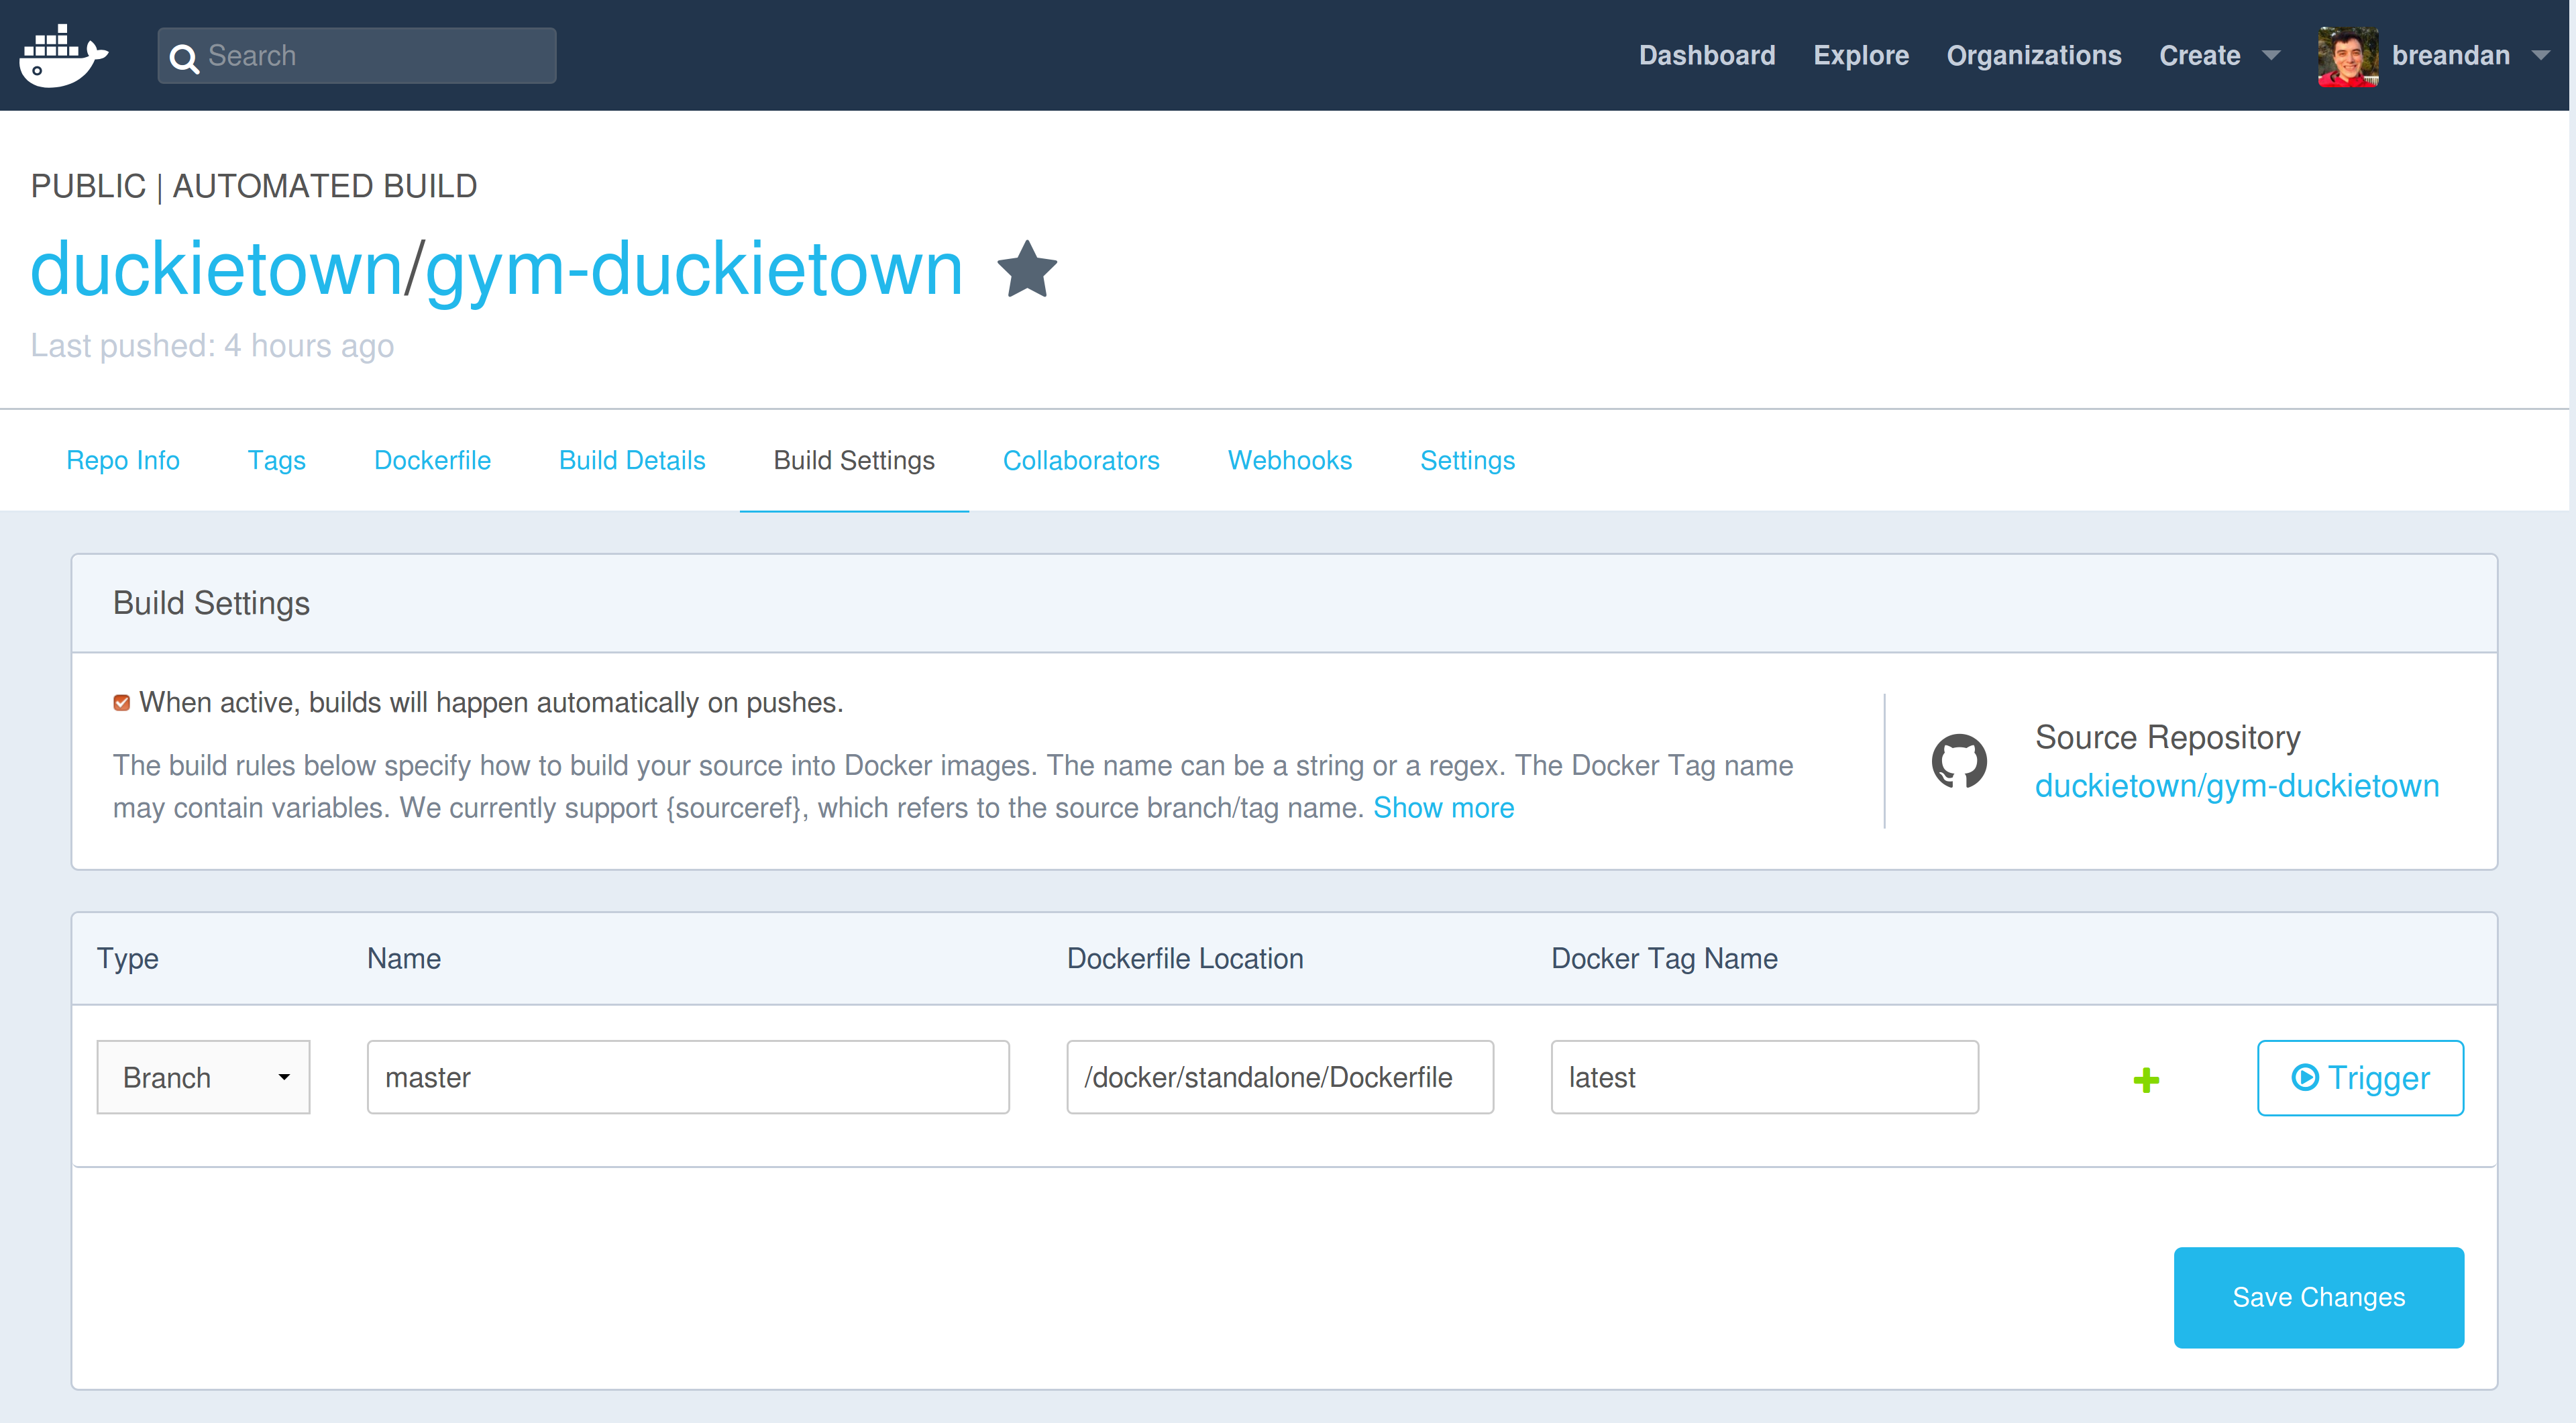
\includegraphics[width=\textwidth]{../figures/docker_hub_autobuild.png}
\end{centering}
%
Le Docker Hub se construit automatiquement et prend en charge la liaison d'un \inline{Dockerfile} dans un dépôt GitHub, et chaque fois que ce \inline{Dockerfile} change, l'image du Docker est mise à jour.

Le Docker Hub dispose également de fonctions permettant de configurer les liens vers les dépôts et les déclencheurs de construction. Ceux-ci reconstruiront automatiquement les images Docker en aval chaque fois qu'un événement se produira.\vspace{10pt}
%
\begin{centering}
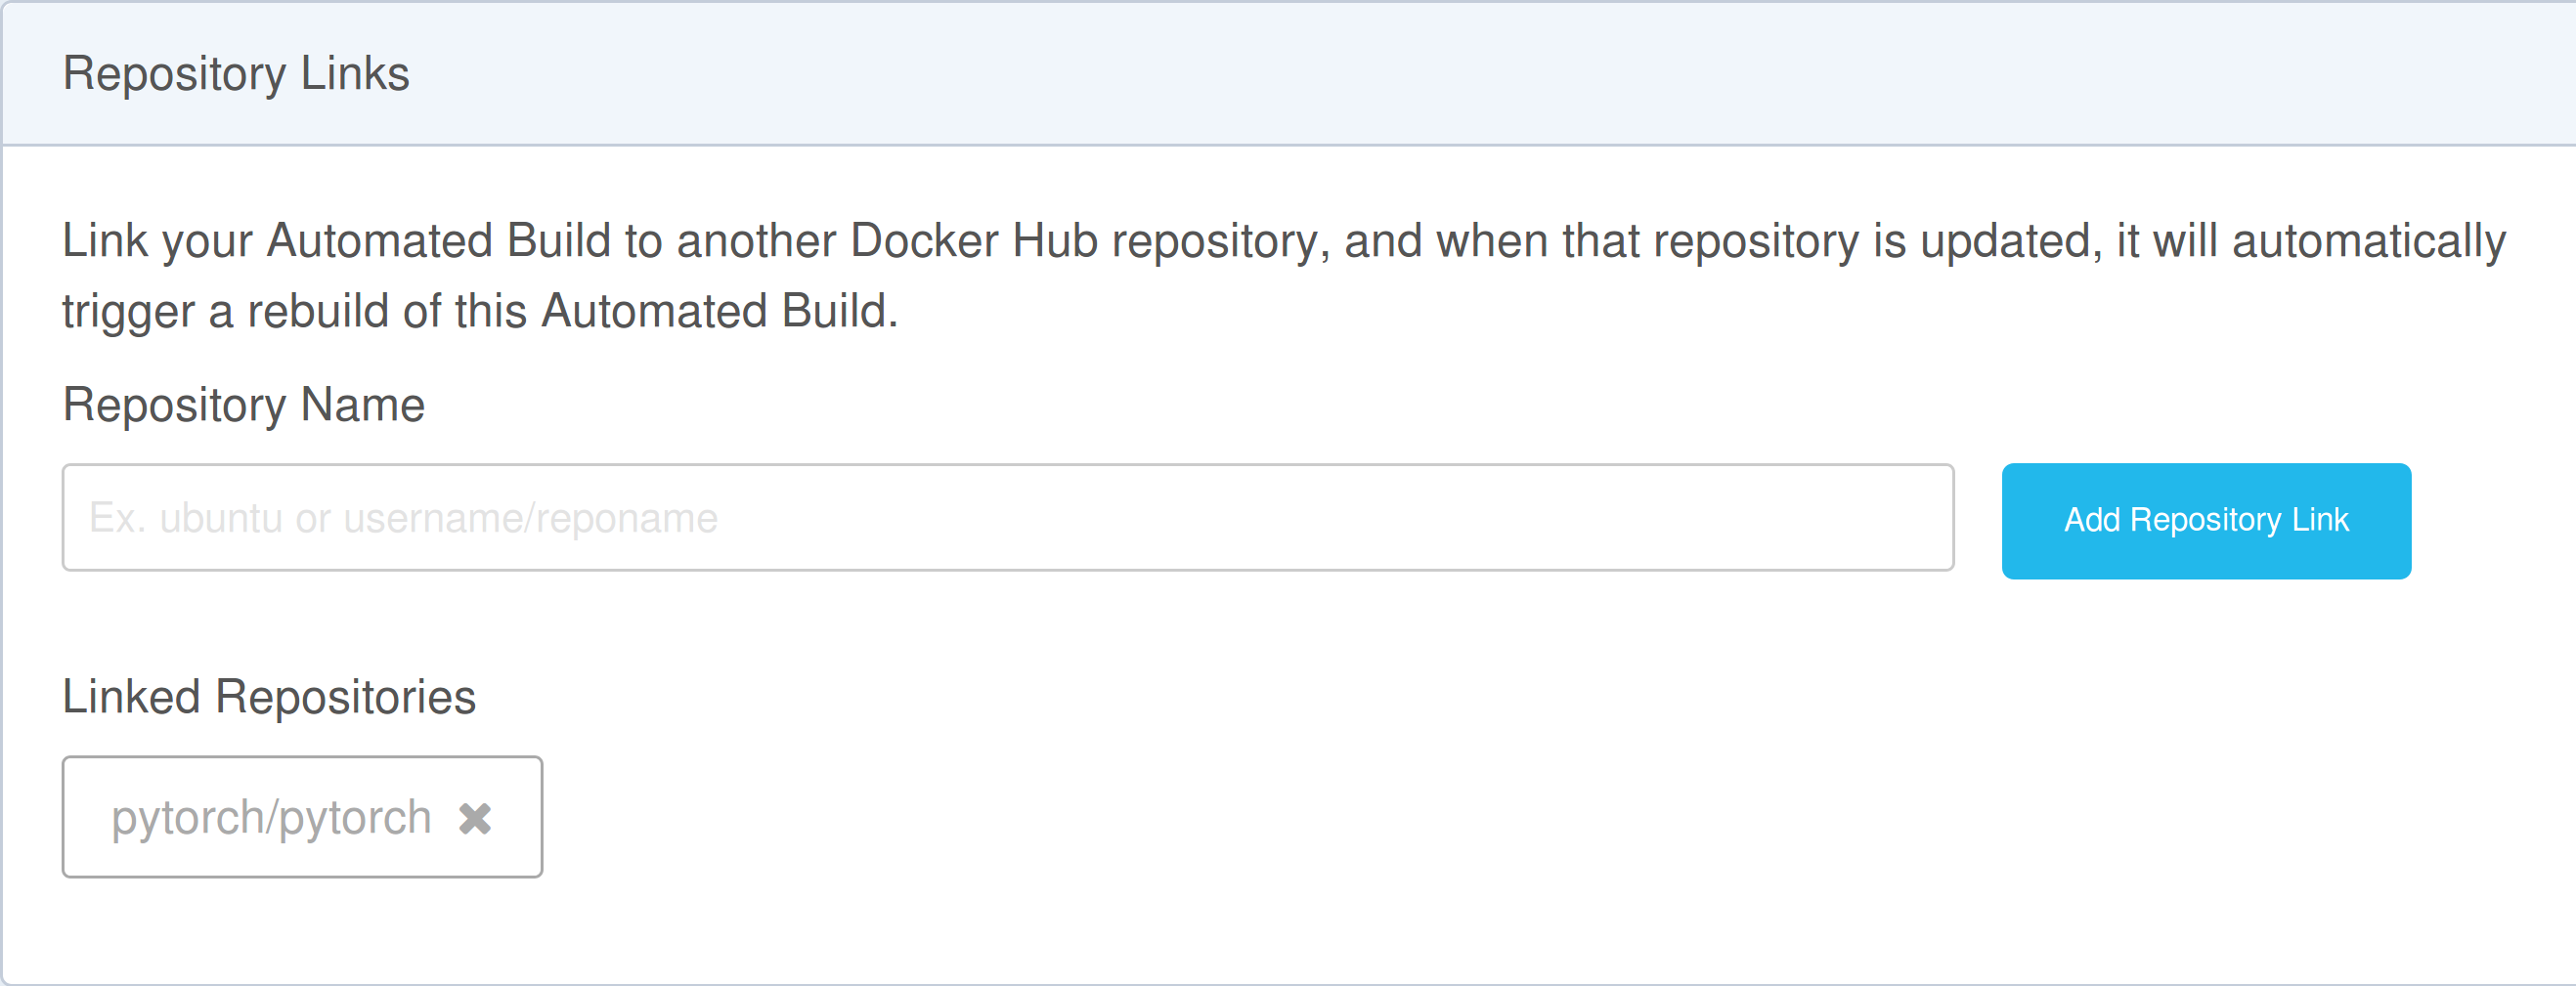
\includegraphics[width=\textwidth]{../figures/docker_hub_repo_links.png}
\end{centering}
%
Les liens vers les dépôts permettent de chaîner les constructions de support entre les dépôts de Docker Hub. Chaque fois qu'un dépôt lié est mis à jour, l'image dépendante est reconstruite.

\subsection{\href{https://cloud.docker.com/}{Docker Cloud}}

Docker Cloud est un registre de dockers qui est entièrement intégré au Docker Hub. Les constructions sont automatiquement publiées de Docker Cloud vers Docker Hub. Les notifications par e-mail et Slack, ainsi que les délais de publication plus longs (jusqu'à 4 heures) sont pris en charge. Docker Cloud prend également en charge des options de compilation plus avancées que Docker Hub, comme un contexte de compilation configurable et des paramètres de cache.

\begin{centering}
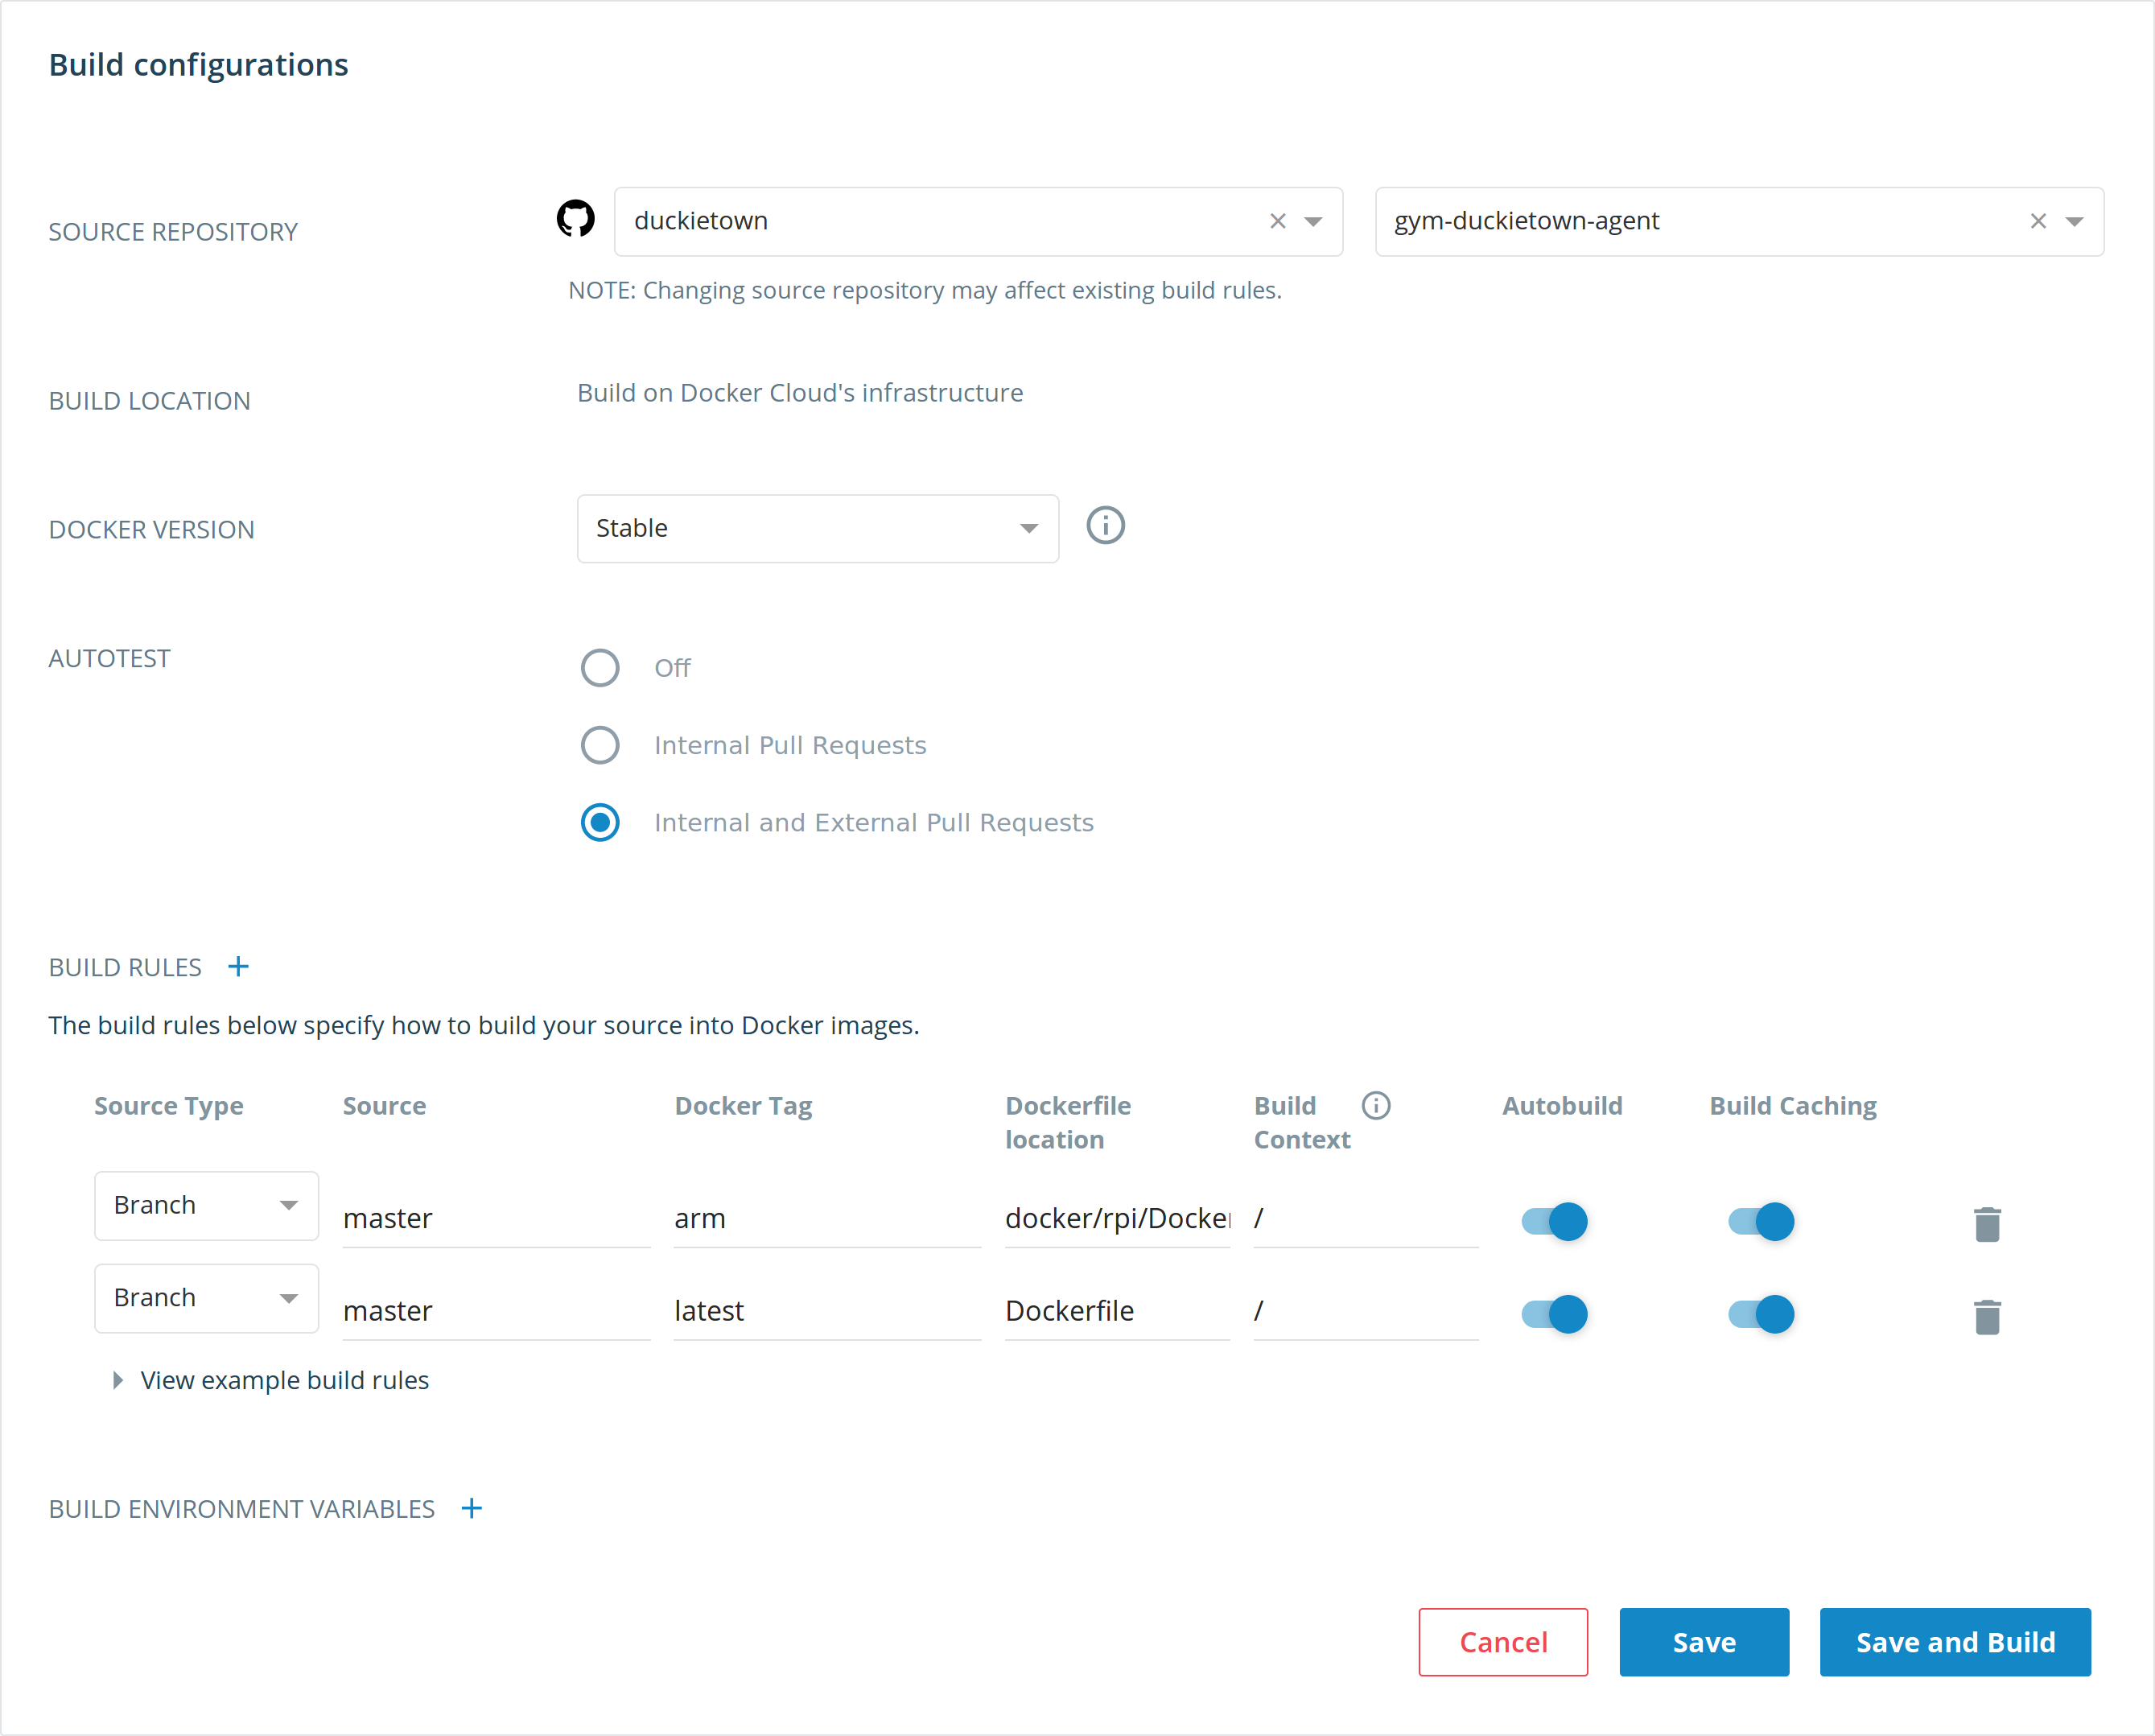
\includegraphics[width=\textwidth]{../figures/docker_cloud.png}
\end{centering}
